\documentclass{article}
\usepackage{graphicx}
\usepackage[margin=1.5cm]{geometry}
\usepackage{amsmath}

\begin{document}

\title{Tuesday Reading Assessment: Chapters 3, 4-1 and 4-2}
\author{Prof. Jordan C. Hanson}

\maketitle

\begin{figure}[ht]
\centering
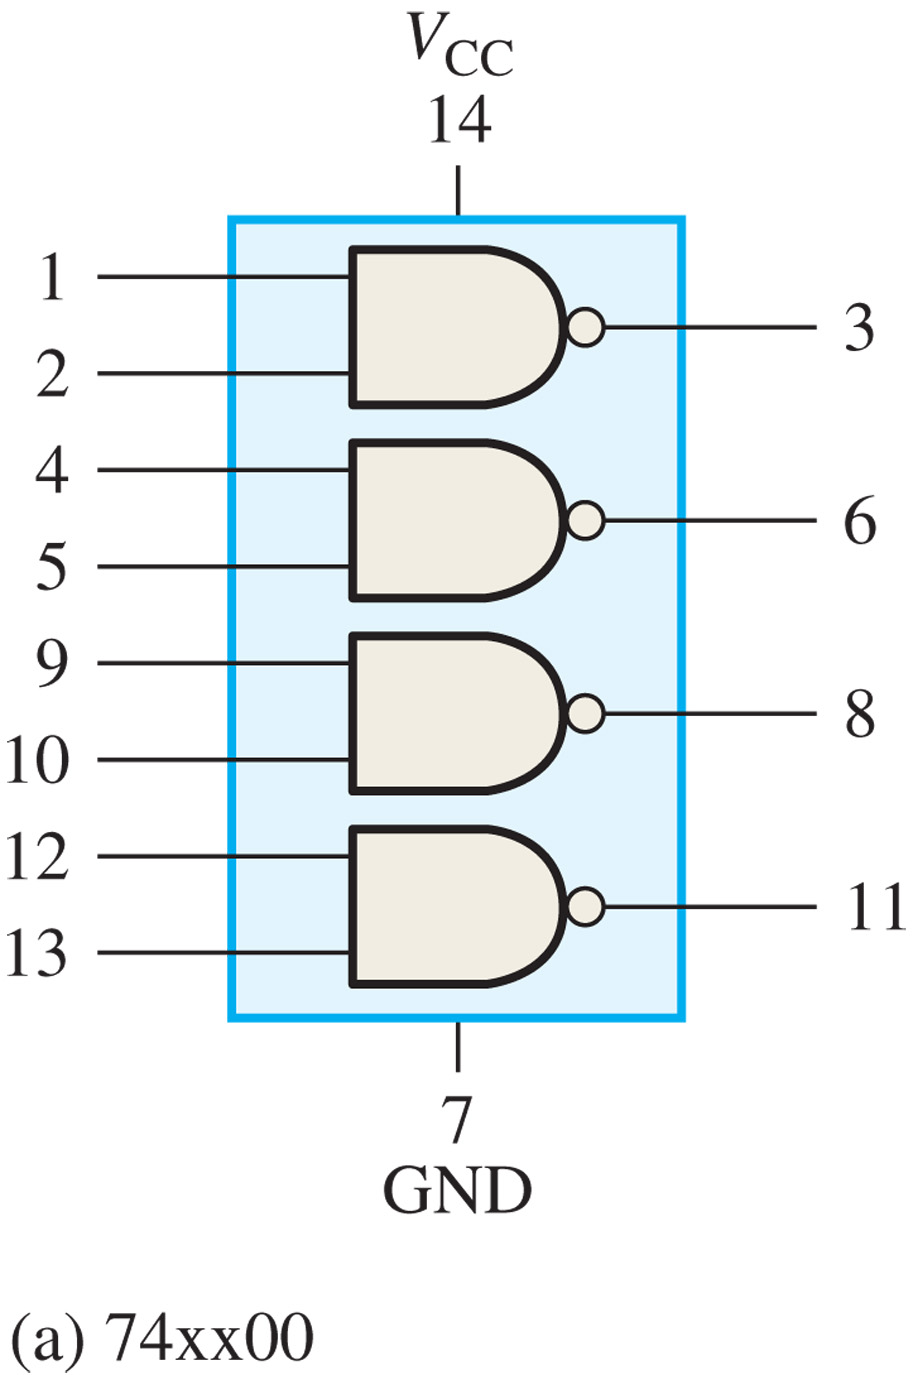
\includegraphics[width=0.15\textwidth]{figures/quad_nand.jpg} \hspace{1cm}
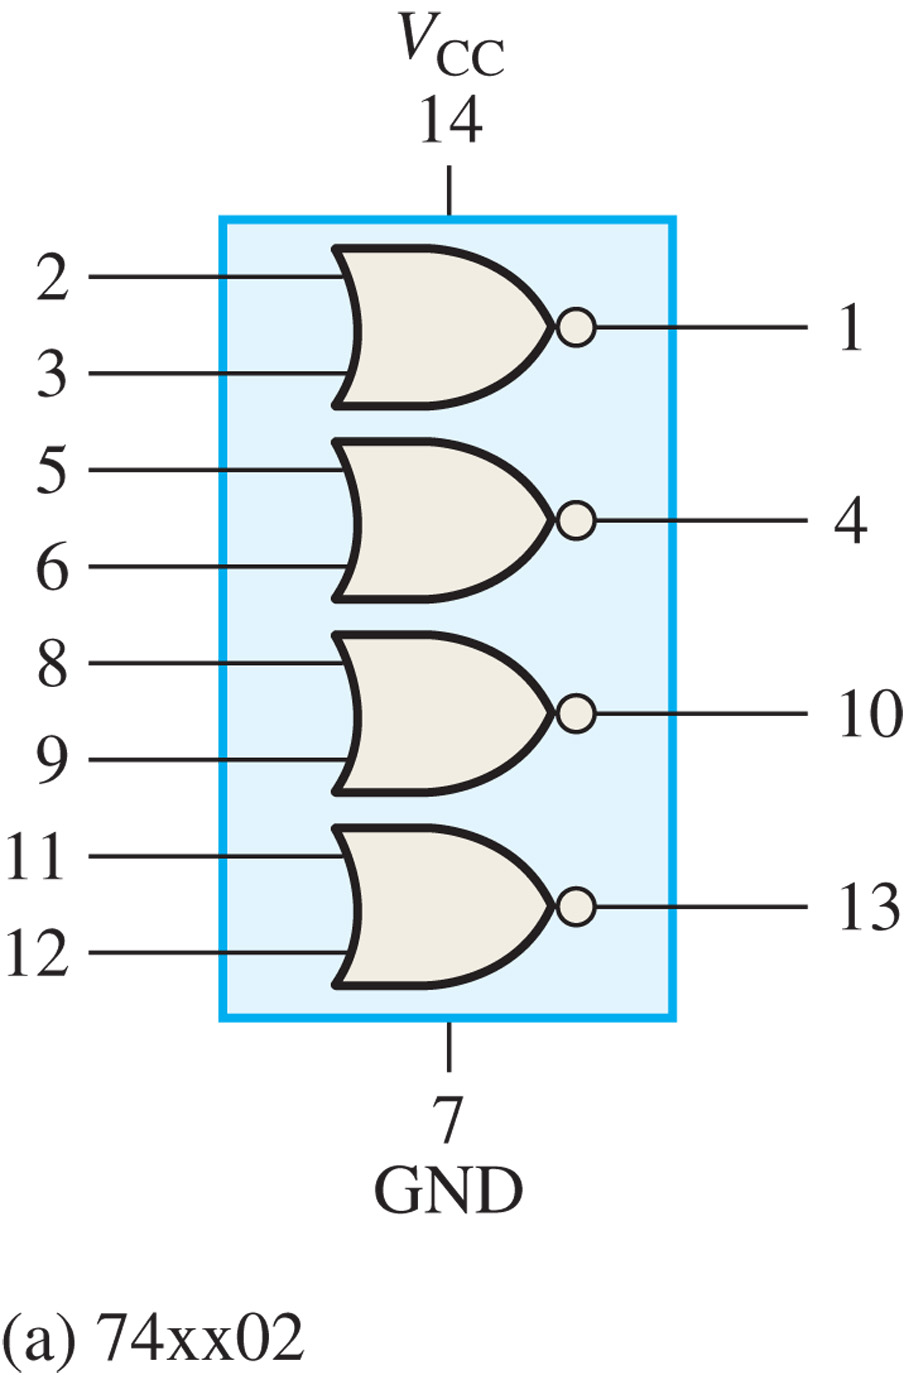
\includegraphics[width=0.15\textwidth]{figures/quad_nor.jpg} \hspace{1cm}
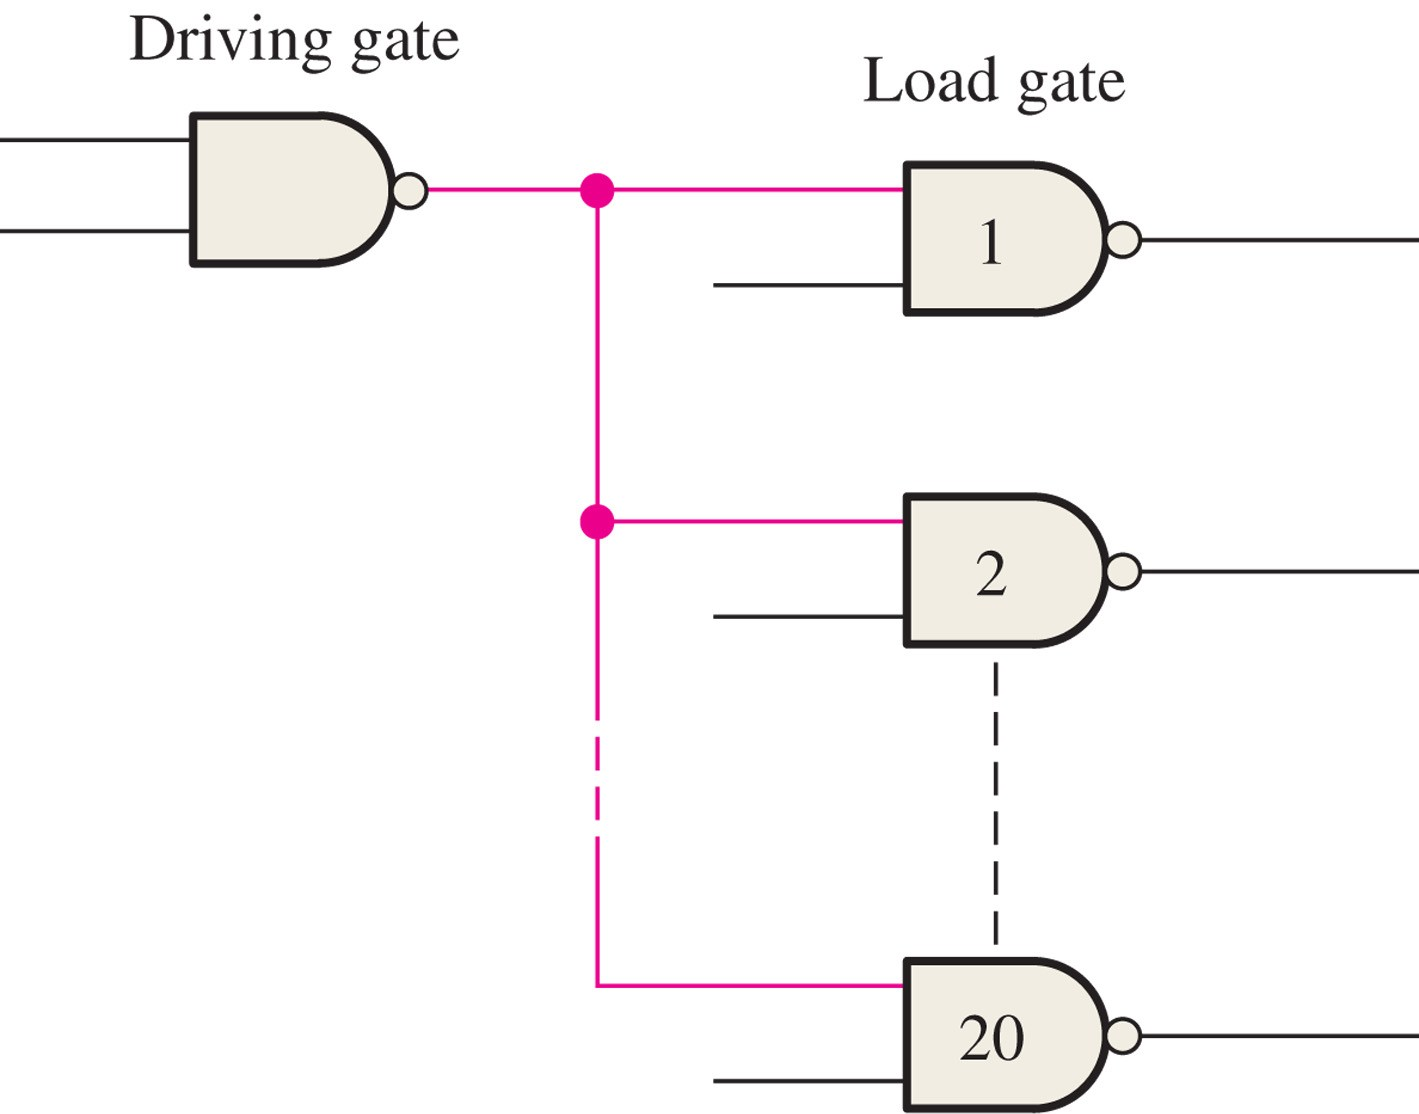
\includegraphics[width=0.3\textwidth]{figures/fan.jpg}
\caption{\label{fig:gates} (Left) A 74xx00 gate, a quad NAND package IC. (Middle) A 74xx02 gate, a quad NOR package IC.}
\end{figure}

\section{Logic Gates and Logic Functions}

\begin{enumerate}
\item Figure \ref{fig:gates} (left) contains a diagram of a quad-NAND IC package, the 74xx00 class.  (a) Create and draw a system of NAND gates that is equivalent to a 2-input AND gate.  (b) Determine a system of connections of outputs to inputs for the 74xx00 IC that will yield one AND gate. (c) Do the same for an OR gate. \\ \vspace{2cm}
\item Repeat the previous exercise with the 74xx02 in Fig. \ref{fig:gates} (middle), a quad-NOR gate. \\ \vspace{1.5cm}
\end{enumerate}

\section{Electrical Characteristics}

\begin{enumerate}
\item Suppose for all individual gates in Fig. \ref{fig:gates} the $I_{\rm CCH} = 10$ $\mu$A, $I_{\rm CCL} = 100$ $\mu$A, and $V_{\rm CC} = 5$ V. (a) What is the power dissipation of your AND gate made from NAND gates? \textit{Hint: $P_{\rm D} = V_{\rm CC}(I_{\rm CCH} + I_{\rm CCL})/2$.} (b) If the \textit{propagation delay time} $t_{\rm P}$ is 5 ns per NAND gate, what is the \textbf{speed power product}, $P_{\rm D}t_{\rm P}$, for the AND gate in pJ? (c) What is the \textit{fan-out} of your AND and OR gate designs from NANDs?  That is, how many gates are driven by the output current of a single gate (see Fig. \ref{fig:gates} (right)).
\end{enumerate}

\end{document}
